\begin{frame}{Aufgabe 7}
  \begin{center}
  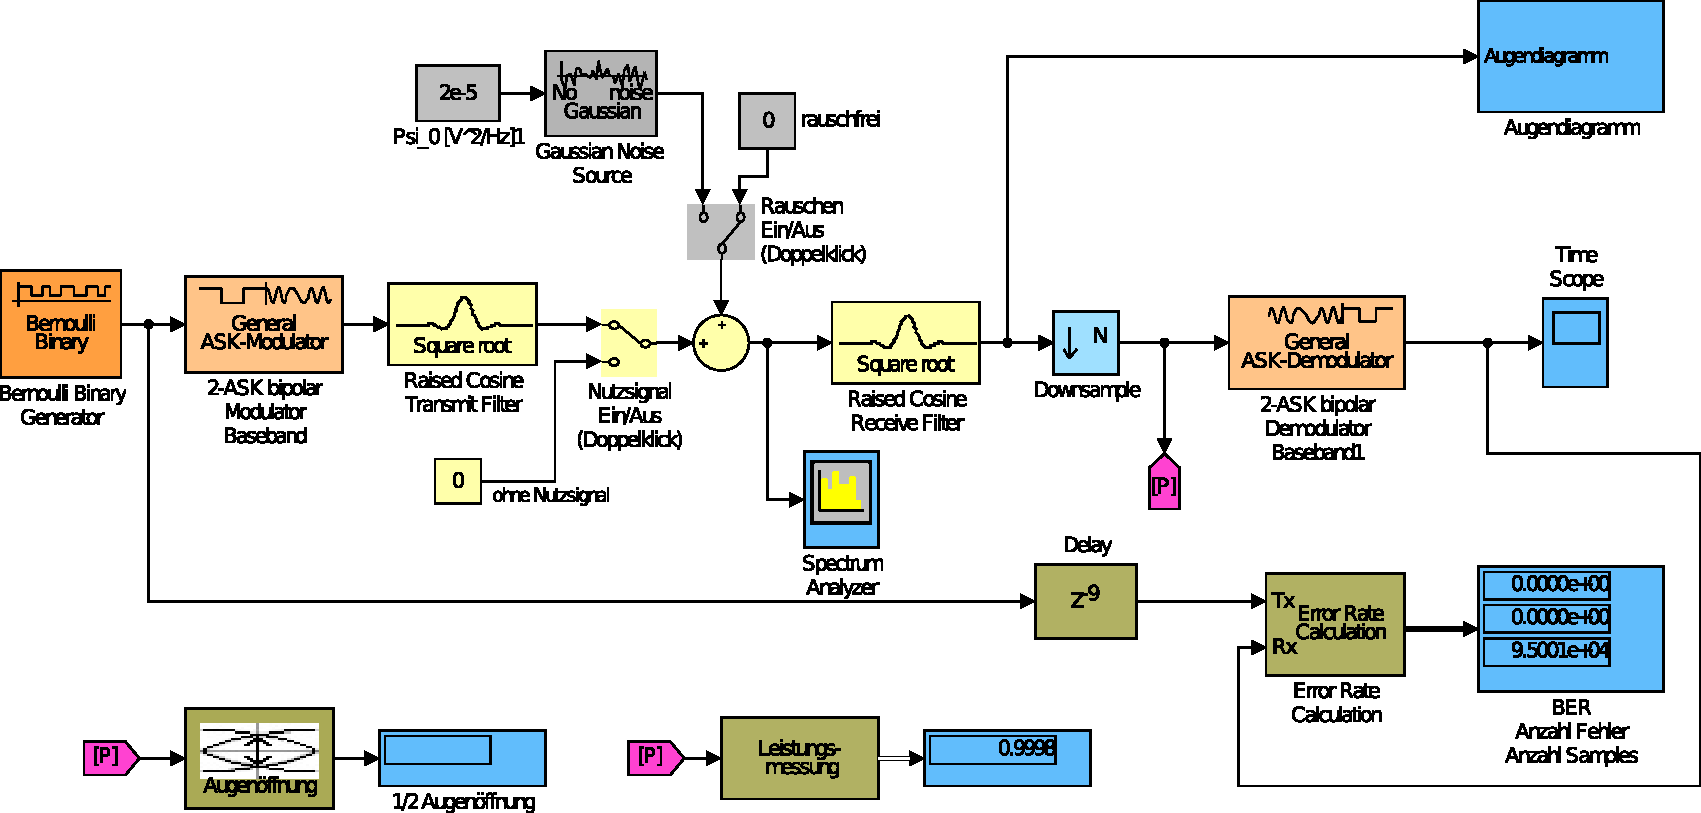
\includegraphics[width=\textwidth]{screenshots/Aufgabe7/modell}
  \end{center}
\end{frame}

\begin{frame}{Aufgabe 7}
  \[g_\mathrm{k}(t) = \frac{1}{\sqrt{5}} \cdot \delta(t)\]
\begin{table}[]
\begin{tabular}{
>{\columncolor{gray0}}l ll}
Kenngröße                          & \cellcolor{gray0}AWGN-Wert & \cellcolor{gray0}A7-Wert \\ \hline
$U_\mathrm{A}$                     & $0.9965 \, \si{\volt}$            & $0.4457 \, \si{\volt}$          \\
$U_\mathrm{R}^2$                   & $0.1 \, \si{\volt}^2$             & $0.1047 \, \si{\volt}^2$        \\
$\rho$                             & $9.93$                            & $1.897$                         \\
$\mathrm{BER}, \mathrm{berechnet}$ & $8.1303 \cdot 10^{-4}$            & $8.42 \cdot 10^{-2}$            \\
$\mathrm{BER}, \mathrm{gemessen}$  & $8.6315 \cdot 10^{-4}$            & $8.024 \cdot 10^{-2}$          
\end{tabular}
\end{table}
\end{frame}